\chapter{Data Definition Language}
\chaptertoc{}
\cleardoubleevenpage
Die Data definition language ist der Teil von SQL, der es ermöglicht, Objekte in der Datenbank zu erstellen und zu verwalten. DDL besteht im wesentlichen aus den vier Befehlen:
\begin{itemize}
    \item \textbf{CREATE}: Erstellen von Objekten
    \item \textbf{ALTER}: Ändern von Objekten
    \item \textbf{DROP}: Objekte löschen
    \item \textbf{TRUNCATE}: Leeren von Tabellen.
\end{itemize}
Der Begriff des \enquote{Objekts} bezieht sich, je nach DBMS, auf die Unterschiedlichsten Dinge:
\begin{itemize}
    \item Tabellen
    \item Views
    \item Indizes
    \item Sequenzen
    \item PL/SQL oder T-SQL Prozeduren und Funktionen
\end{itemize}
\dots und vieles mehr. Welche Möglichkeiten dem Anwender bei der Erstellung eines Objekts geboten werden, ist stark abhängig vom jeweiligen DBMS.
\section{Tabellen erstellen und verwalten}
\subsection{Namenskonventionen und Einschränkungen}
Bevor näher auf die Namenskonventionen für Objekte eingegangen wird, müssen an dieser Stelle zuerst einige Fachbegriffe geklärt werden.
\begin{itemize}
    \item \textbf{Bezeichner}: Namen für Objekte (Tabellen, Spalten, Views, usw.) heißen im Fachjargon Bezeichner.
    \item \textbf{Umschlossene Bezeichner}: Sind Bezeichner, die in Anführungszeichen \char34{} eingeschlossen sind
    \item \textbf{Reservierte Wörter}: Begriffe die in SQL eine bestimmte Bedeutung haben, z. B. \SELECT , \WHERE , usw.
    \item \textbf{Namensraum}: Logische Einteilung für Objektnamen. Bezeichner müssen innerhalb eines Namensraumes eindeutig sein.
\end{itemize}
\tabelle{createtablerestrictions} listet die wichtigsten
Einschränkungen auf, die für Bezeichner in beiden DBMS gelten.
\begin{center}
    \tablecaption{Einschränkungen für Bezeichner}
    \label{createtablerestrictions}
    \begin{small}
        \tablefirsthead{
            \multicolumn{1}{c}{\textbf{}} &
            \multicolumn{1}{c}{\textbf{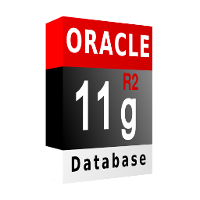
\includegraphics[scale=1]{oracle_11g}}} &
            \multicolumn{1}{c}{\textbf{
\includegraphics[scale=1]{ms_sql}}} \\
            \hline
        }
        \tablehead{
            \multicolumn{1}{c}{\textbf{Einschränkung}} &
            \multicolumn{1}{c}{\textbf{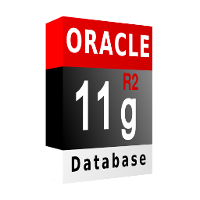
\includegraphics[scale=1]{oracle_11g}}} &
            \multicolumn{1}{c}{\textbf{
\includegraphics[scale=1]{ms_sql}}} \\
            \hline
        }
        \tabletail{
            \hline
        }
        \tablelasttail{
            \hline
        }
        \begin{supertabular}{|l|p{5.5cm}|p{5.7cm}|}
            \textbf{Bezeichnerlänge} & 30 & 128\\
            \hline
            \textbf{Reservierte Wörter} & Bezeichner können keine reservierten Wörter sein, es sei denn, sie sind in Anführungszeichen \char34{} eingeschlossen. & Bezeichner können keine reservierten Wörter sein, es sei denn, sie sind in Anführungszeichen \char34{} eingeschlossen. \\
            \hline
            \textbf{Namensgebung} & Wenn Bezeichner nicht in Anführungszeichen (\char34{}) einschlossen sind, müssen diese mit einem Buchstaben beginnen. Für umschlossene Bezeichner gilt dies nicht. & Wenn Bezeichner nicht in Anführungszeichen (\char34{}) oder ([]) einschlossen sind, müssen diese mit einem Buchstaben, \_, @ oder \# beginnen. Für umschlossene Bezeichner gilt dies nicht. \\
            \hline
            \textbf{Gültige Zeichen} & Nicht umschlossene Bezeichner können nur aus den Buchstaben a-z und A-Z, den Ziffern 0-9, sowie \_, \$ und \# bestehen. Für umschlossene Bezeichner gilt, dass dort alle Zeichen, auch Leerzeichen vorkommen können. & Nicht umschlossene Bezeichner können nur aus den Buchstaben a-z und A-Z, den Ziffern 0-9, sowie @, \$, \_ und \# bestehen. Für umschlossene Bezeichner gilt, dass dort alle Zeichen, auch Leerzeichen vorkommen können. \\
            \hline
            \textbf{Namensgleichheit} & Zwei Datenbankobjekte im gleichen Namensraum müssen unterschiedliche Namen haben.  & Bezeichner müssen innerhalb eines Schemas eindeutig sein.\\
            \hline
            \textbf{Casesensitivität} & Nicht umschlossene Bezeichner sind nicht Casesensitiv. Bezeichner die mit (\char34{}) oder ([]) umschlossen sind, sind Casesensitiv. & Bezeichner die mit (\char34{}) oder ([]) umschlossen sind, sind nicht Casesensitiv. \\
        \end{supertabular}
    \end{small}
\end{center}
\begin{merke}
    Damit umschlossene Bezeichner in SQL Server 2008 R2 genutzt werden können, muss die Option \textit{QUOTED\_IDENTIFIER} den Wert \textit{ON} haben. Dieser kann nötigenfalls mit \languagemssql{SET QUOTED_IDENTIFIER ON} gesetzt werden.
\end{merke}
\clearpage
Die folgenden Internetliteraturhinweise liefern weitere Informationen.
\begin{literaturinternet}
    \item \cite{i27561}
    \item \cite{ms187879}
\end{literaturinternet}
\subsection{CREATE TABLE - Tabellen erstellen}
Sowohl in Oracle als auch in SQL Server werden Tabellen mit Hilfe des
Kommandos \languageorasql{CREATE TABLE} erstellt. Die grundlegende,
SQL-Standardkonforme Syntax für \languageorasql{CREATE TABLE} lautet:
\begin{lstlisting}[language=oracle_sql,caption={Die Syntax der CREATE TABLE-Anweisung},label=sql08_01]
CREATE TABLE <tabellen_name> (
  <spaltenbezeichner 1> <datentyp>,
  <spaltenbezeichner 2> <datentyp>,
  ...,
  <spaltenbezeichner n> <datentyp>
);
        \end{lstlisting}
\begin{center}
    \tablecaption{Die CREATE TABLE-Anweisung}
    \label{createtablesyntax}
    \begin{small}
        \tablefirsthead{
            \multicolumn{1}{c}{\textbf{Ausdruck}} &
            \multicolumn{1}{c}{\textbf{Bedeutung}} \\
            \hline
        }
        \tablehead{
            \multicolumn{1}{c}{\textbf{Ausdruck}} &
            \multicolumn{1}{c}{\textbf{Bedeutung}} \\
            \hline
        }
        \tabletail{
            \hline
        }
        \begin{supertabular}{|l|p{9.45cm}|}
            CREATE TABLE <Tabellenname> & Diese Klausel leitet das Erstellen der Tabelle ein. Für den Tabellennamen gelten die in \tabelle{createtablerestrictions} angegebenen Beschränkungen. \\
            \hline
            <Spaltenbezeichner> <Datentyp> & Jede Tabellenspalte wird durch einen Bezeichner/Name und einen Datentyp repräsentiert. Mit Hilfe des Namens kann die Spalte später angesprochen werden und der Datentyp legt den Wertebereich der Spalte fest. Je nach DBMS gelten auch hier unterschiedliche Einschränkungen. \\
        \end{supertabular}
    \end{small}
\end{center}
\beispiel{sql08_02} zeigt ein einfaches \languageorasql{CREATE TABLE}-Statement.
\begin{lstlisting}[language=oracle_sql,caption={Eine einfache CREATE TABLE-Anweisung in Oracle},label=sql08_02]
CREATE TABLE Aktie (
  Aktie_ID  NUMBER,
  Name      VARCHAR2(25),
  WKN       NUMBER,
  ISIN      VARCHAR2(12)
);
        \end{lstlisting}
\clearpage
\begin{lstlisting}[language=ms_sql,caption={Das gleiche in MS SQL Server},label=sql08_03]
CREATE TABLE Aktie (
  Aktie_ID  NUMERIC,
  Name      VARCHAR(25),
  WKN       NUMERIC,
  ISIN      VARCHAR(12)
);
        \end{lstlisting}
Es wird eine Tabelle namens \identifier{Aktie}, mit den Spalten \identifier{Aktie\_ID}, \identifier{Name}, \identifier{WKN} und \identifier{ISIN} angelegt.

Zur besseren Umsetzung der Beispiele in den folgenden Abschnitten, werden nun einige Datensätze in die Tabelle \identifier{Aktie} eingefügt.
\begin{lstlisting}[language=oracle_sql,caption={Beispieldatensätze},label=sql08_04]
INSERT INTO Aktie
VALUES (1, 'Henker Co KG', 1236547, 'DE0006800002');

INSERT INTO Aktie
VALUES (2, 'AD and D', 43116589, 'DE0002300023');

COMMIT;
        \end{lstlisting}
\subsection{CREATE TABLE AS... (CTAS)}
Die Abkürzung \enquote{CTAS} steht für \languageorasql{CREATE TABLE AS} und meint ein \languageorasql{CREATE TABLE} mit Unterabfrage. Mit Hilfe von CTAS können bestehende Tabellen teilweise oder ganz kopiert werden. \beispiel{sql08_05} zeigt, wie in Oracle eine vollständige Kopie der Tabelle \identifier{Aktie} angefertigt wird.
\begin{lstlisting}[language=oracle_sql,caption={Oracle - CREATE TABLE AS (CTAS)},label=sql08_05]
CREATE TABLE Aktie_Kopie
AS
  SELECT *
  FROM   Aktie;
        \end{lstlisting}
Es wird eine Tabelle namens \identifier{Aktie\_Kopie} erstellt. Diese erhält die komplette Struktur und den gesamten Inhalt der Tabelle \identifier{Aktie}.

In Microsoft SQL Server kennt das \languagemssql{CREATE TABLE}-Statement keine Möglichkeit, eine Unterabfrage zu nutzen. Hier muss stattdessen das \languagemssql{SELECT INTO}-Statement genutzt werden.
\begin{lstlisting}[language=ms_sql,caption={MS SQL Server - SELECT INTO},label=sql08_06]
SELECT *
INTO   Aktie_Kopie
FROM   Aktie;
        \end{lstlisting}
Die Auswirkungen bleiben die gleichen, wie unter Oracle mit CTAS.

\begin{merke}
    Microsoft SQL Server kennt das \languagemssql{CREATE TABLE AS}-Statement nicht. Es muss stattdessen das \languagemssql{SELECT INTO}-Statement genutzt werden. Die Auswirkungen von \languagemssql{CREATE TABLE AS} und \languagemssql{SELECT INTO} sind gleich.
\end{merke}
\subsection{ALTER TABLE - Tabellen verändern}
Mit Hilfe der \languageorasql{ALTER TABLE}-Anweisung können bestehende Tabellendefinition verändert werden. Dies betrifft z. B.:
\begin{itemize}
    \item Das Hinzufügen neuer Spalten zu einer Tabelle.
    \item Das Löschen von Spalten.
    \item Das Umbenennen von Spalten.
    \item Das Ändern des Datentyps einer Spalte.
    \item Ändern der Größe einer Spalte.
    \item Das Hinzufügen, ändern und löschen eines Standardwerts.
    \item Das Hinzufügen und Löschen von Constraints (siehe \abschnitt{constraints1})
\end{itemize}
\subsubsection{Eine neue Spalte an eine Tabelle anfügen}
In beiden DBMS gibt es, zum Hinzufügen einer Spalte zu einer Tabelle, die \lstinline{ADD}-Klausel des \languageorasql{ALTER TABLE}-Kommandos. In \beispiel{sql08_07}, wird der Tabelle \identifier{Aktie} eine neue Spalte namens \identifier{Herkunft} hinzugefügt.
\begin{lstlisting}[language=oracle_sql,caption={Oracle - Tabellenspalte hinzufügen},label=sql08_07]
ALTER TABLE Aktie
ADD Herkunft VARCHAR2(25);
          \end{lstlisting}
In SQL Server unterscheidet sich dieses Statement nur durch den Datentyp.
\clearpage
\begin{lstlisting}[language=ms_sql,caption={MS SQL Server - Tabellenspalte hinzufügen},label=sql08_08]
ALTER TABLE Aktie
ADD Herkunft VARCHAR(25);
          \end{lstlisting}
\begin{merke}
    Wird eine neue Spalte an eine Tabelle angefügt, haben alle Zellen dieser Spalte den Wert NULL, es sei den, es wird ein Standardwert für diese Spalte definert. In diesem Falle füllt Oracle die Spalte mit dem Standardwert auf. SQL Server tut dies nicht.
\end{merke}
\beispiel{sql08_09} und \beispiel{sql08_10} zeigen, wie sich Oracle und MS SQL Server verhalten, wenn eine neue Spalte, mit einem Standardwert, hinzugefügt wird. Die Spalte \identifier{Herkunft} wird mit dem Standardwert \enquote{Deutschland} an die Tabelle \identifier{Aktie} angefügt. In Oracle werden dann automatisch alle bereits vorhandenen Zeilen mit dem neuen Standardwert aufgefüllt. In SQL Server wird dies nicht der Fall sein.

\begin{lstlisting}[language=oracle_sql,caption={Tabellenspalte mit Standardwert hinzufügen in Oracle},label=sql08_09]
ALTER TABLE Aktie
ADD Herkunft VARCHAR2(25) DEFAULT 'Deutschland';

SELECT *
FROM   Aktie;
          \end{lstlisting}
\begin{center}
    \begin{small}
        \changefont{pcr}{m}{n}
        \tablefirsthead {
            \multicolumn{1}{r}{\textbf{AKTIE\_ID}} &
            \multicolumn{1}{l}{\textbf{NAME}} &
            \multicolumn{1}{l}{\textbf{WKN}} &
            \multicolumn{1}{l}{\textbf{ISIN}} &
            \multicolumn{1}{l}{\textbf{HERKUNFT}} \\
            \cmidrule(r){1-1}\cmidrule(l){2-2}\cmidrule(l){3-3}\cmidrule(l){4-4}\cmidrule(l){5-5}
        }
        \tablehead{}
        \tabletail {
            \multicolumn{5}{l}{\textbf{2 Zeilen ausgewählt}} \\
        }
        \tablelasttail {
            \multicolumn{5}{l}{\textbf{2 Zeilen ausgewählt}} \\
        }
        \begin{oraclesql}
            \begin{supertabular}{rllll}
                1 & Henker Co KG & 1236547 & DE0006800002 & Deutschland \\
                2 & AD and D & 43116589 & DE0002300023 & Deutschland \\
            \end{supertabular}
        \end{oraclesql}
    \end{small}
\end{center}

Wird das gleiche Experiment in MS SQL Server durchgeführt, zeigt sich das die Spalte \identifier{Herkunft} nicht automatisch aufgefüllt wird.
\begin{lstlisting}[language=ms_sql,caption={Tabellenspalte mit Standardwert hinzufügen in SQL Server},label=sql08_10]
ALTER TABLE Aktie
ADD Herkunft VARCHAR(25) DEFAULT 'Deutschland';

SELECT *
FROM   Aktie;
          \end{lstlisting}
\clearpage
\begin{center}
    \begin{small}
        \changefont{pcr}{m}{n}
        \tablefirsthead {
            \multicolumn{1}{l}{\textbf{AKTIE\_ID}} &
            \multicolumn{1}{l}{\textbf{NAME}} &
            \multicolumn{1}{l}{\textbf{WKN}} &
            \multicolumn{1}{l}{\textbf{ISIN}} &
            \multicolumn{1}{l}{\textbf{HERKUNFT}} \\
            \cmidrule(l){1-1}\cmidrule(l){2-2}\cmidrule(l){3-3}\cmidrule(l){4-4}\cmidrule(l){5-5}
        }
        \tablehead{}
        \tabletail {
            \multicolumn{5}{l}{\textbf{2 Zeilen ausgewählt}} \\
        }
        \tablelasttail {
            \multicolumn{5}{l}{\textbf{2 Zeilen ausgewählt}} \\
        }
        \begin{oraclesql}
            \begin{supertabular}{lllll}
                1 & Henker Co KG & 1236547 & DE0006800002 &  NULL \\
                2 & AD and D & 43116589 & DE0002300023 & NULL \\
            \end{supertabular}
        \end{oraclesql}
    \end{small}
\end{center}
\subsubsection{Spalten vergrößern und verkleinern}
Es besteht die Möglichkeit, die Definition einer Spalte nachträglich zu verändern. Dabei können verschiedene Dinge, wie z. B. der Spaltendatentyp oder der Standardwert einer Spalte geändert werden. Um eine solche Änderung durchzuführen, kennt das \languageorasql{ALTER TABLE}-Kommando unter Oracle die \languageorasql{MODIFY}-Klausel und unter SQL Server die \languagemssql{ALTER COLUMN}-Klausel. Hierzu einige Beispiele.

In \beispiel{sql08_11} wird die Breite der Spalte \identifier{Herkunft} in der Tabelle \identifier{Aktie} verändert.
\begin{lstlisting}[language=oracle_sql,caption={Anpassen der Spaltenlänge in Oracle},label=sql08_11]
ALTER TABLE Aktie
MODIFY Herkunft VARCHAR2(30);
          \end{lstlisting}
Eine Vergrößerung stellt prinzipiell niemals ein Problem dar. Schwieriger wird es hingegen, wenn eine Spalte verkleinert werden muss. In Oracle geht das nur dann, wenn die Inhalte der Spalte kleiner sind als die neue Spaltengröße. Anderenfalls antwortet Oracle mit der in \beispiel{sql08_12} sichtbaren Fehlermeldung:
\begin{lstlisting}[language=oracle_sql,caption={Fehlermeldung beim verkleinern einer Spalte in Oracle},label=sql08_12]
MODIFY Herkunft VARCHAR2(15)
       *
FEHLER in Zeile 2:
ORA-01441: Spaltenlaenge kann nicht vermindert werden, weil ein Wert zu gross
ist
          \end{lstlisting}
\begin{merke}
    Eine Tabellenspalte kann in Oracle nur auf die Größe des größten darin enthaltenden Werts verkleinert werden. In SQL Server kann eine Tabellenspalte auch mit Inhalt verkleinert werden.
\end{merke}
Bei SQL Server muss lediglich die \languageorasql{MODIFY}-Klausel durch die \languagemssql{ALTER COLUMN}-Klausel ersetzt werden.
\begin{lstlisting}[language=ms_sql,caption={Anpassen der Spaltenlänge in SQL Server},label=sql08_13]
ALTER TABLE Aktie
ALTER COLUMN Herkunft VARCHAR(30);
          \end{lstlisting}
\subsubsection{Ändern des Datentyps}
Mit Hilfe der \languageorasql{MODIFY}-Klausel kann nicht nur die Größe einer Spalte verändert werden, sondern auch der Datentyp. In \beispiel{sql08_14} wird der Datentyp der Spalte \identifier{WKN} von \languageorasql{NUMBER} auf \languageorasql{VARCHAR2}, bzw. von \languagemssql{NUMERIC} auf \languagemssql{VARCHAR} geändert.
\begin{lstlisting}[language=oracle_sql,caption={Ändern des Datentyps},label=sql08_14]
ALTER TABLE Aktie
MODIFY WKN VARCHAR2(10);
          \end{lstlisting}
In SQL Server sieht das Ändern des Datentyps einer Spalte sehr ähnlich aus.
\begin{lstlisting}[language=ms_sql,caption={Ändern des Datentyps},label=sql08_15]
ALTER TABLE Aktie
ALTER COLUMN WKN VARCHAR(10);
          \end{lstlisting}
\begin{merke}
    Eine Tabellenspalte muss in Oracle leer sein, damit ihr Datentyp verändert werden kann. In SQL Server kann der Datentyp einer Spalte auch mit Inhalt verändert werden.
\end{merke}
\subsubsection{Einen Defaultvalue hinzufügen}
Eine weitere Aktion die mit \languageorasql{MODIFY} bzw. \languagemssql{ALTER COLUMN} möglich ist, ist das Hinzufügen, ändern oder entfernen eines Standardwertes bei einer Tabellenspalte. In \beispiel{sql08_16} wird in Oracle der Standardwert der Spalte \identifier{Herkunft} von \enquote{Deutschland} auf \enquote{USA} geändert.
\begin{lstlisting}[language=oracle_sql,caption={Einen Standardwert ändern},label=sql08_16]
ALTER TABLE Aktie
MODIFY Herkunft DEFAULT 'USA';
          \end{lstlisting}
Mit der gleichen Anweisung kann der Standardwert eine Spalte, unter Oracle, nicht nur geändert sondern auch hinzugefügt werden. Das Löschen des Standardwertes geschieht, indem NULL als Standardwert zugewiesen wird.
\begin{lstlisting}[language=oracle_sql,caption={Standardwert hinzufügen},label=sql08_17]
ALTER TABLE Aktie
MODIFY Herkunft DEFAULT NULL;
          \end{lstlisting}
Bei SQL Server ist das Löschen eines Standardwerts anders als bei
Oracle. In SQL Server wird ein Standardwert als sogenanntes
Constraint\footnote{constraint engl. = Einschränkung} gehandhabt.
Deshalb wird diese Aktion zu einem späteren Zeitpunkt in
\abschnitt{sqlserverdefaultconstraint} behandelt.

\begin{merke}
    Wird in Oracle mit Hilfe \languageorasql{ADD}-Klausel eine Spalte
    mit Standardwert hinzugeügt, werden alle NULL-Werte in der
    gleichen Spalte mit dem Standardwert aufgefüllt. Wird die Spalte
    dagegen mit der \languageorasql{MODIFY}-Klausel, nachträglich mit
    einem Default-Wert ausgestattet, bleiben alle NULL-Werte erhalten!
\end{merke}

\subsubsection{Tabellenspalten umbenennen}
Es ist möglich, bestehende Spalten umzubenennen. Dafür wird in
Oracle die \languageorasql{RENAME COLUMN}-Klausel des
\languageorasql{ALTER TABLE}-Kommandos verwendet. In Microsoft SQL
Server gibt es hierfür eine gespeicherte Hilfsprozedur, welche das
Umbenennen übernimmt. Der neue Spaltenname muss innerhalb der
Tabelle eindeutig sein und es dürfen keine anderen Operationen
zusammen mit dem Umbenennen geschehen.
\begin{lstlisting}[language=oracle_sql,caption={Tabellenspalte umbenennen in Oracle},label=sql08_18]
ALTER TABLE Aktie
RENAME COLUMN Name TO Bezeichnung;
          \end{lstlisting}
\begin{lstlisting}[language=ms_sql,caption={Tabellenspalte umbenennen in SQL Server},label=sql08_19, emphstyle={[9]\color{red}},emph={[9]sp_rename}]
EXEC sp_rename 'Aktie.Name', 'Bezeichnung', 'COLUMN'
          \end{lstlisting}
\begin{merke}
    Für das Umbenennen von Objekten ist in SQL Server die gespeicherte
    Hilfsprozedur \languagemssql{sp\_rename} zuständig.
\end{merke}
Zu beachten ist, dass das Umbenennen einer Spalte Auswirkungen auf
abhängige Objekte wie z. B. Views oder Trigger haben kann und
deshalb mit größter Vorsicht durchzuführen ist.
\subsubsection{Tabellenspalten löschen}
Tabellenspalten, die nicht mehr benötigt werden, können jeder
Zeit gelöscht werden. Auf diese einfache Art und Weise kann
Speicherplatz zu weiteren Nutzung freigegeben werden. Allgemein gilt
als Einschränkung beim Löschen einer Tabellenspalte:
\begin{itemize}
    \item Die letzte Spalte in einer Tabelle kann nicht gelöscht
          werden. Es muss dann die gesamte Tabelle gelöscht werden.
\end{itemize}
Für Oracle gilt zusätzlich:
\begin{itemize}
    \item Ein normaler Nutzer kann keine Spalten aus einer Tabelle
          löschen, die dem Nutzer sys gehört.
\end{itemize}
\beispiel{sql08_19} zeigt das Löschen einer Tabellenspalte in Oracle und SQL Server.
\begin{lstlisting}[language=oracle_sql, caption={Tabellenspalte
          löschen},label=sql08_20]
ALTER TABLE Aktie
DROP COLUMN WKN;
          \end{lstlisting}
\subsection{DROP TABLE - Tabellen löschen}
Eine nicht mehr benötigte Tabelle, wird in Oracle und SQL Server mit dem \languageorasql{DROP TABLE}-Kommando gelöscht.
\begin{itemize}
    \item Alle verknüpften Indizes und Trigger werden mitgelöscht.
    \item Alle abhängigen Views bleiben bestehen und werden ungültig.
\end{itemize}
Das folgende Beispiel löscht die Tabelle \identifier{Aktie}.
\begin{lstlisting}[language=oracle_sql,caption={Eine Tabelle löschen},label=sql08_21]
DROP TABLE Aktie;
        \end{lstlisting}
\subsection{TRUNCATE TABLE - Tabellen leeren}
Eine Tabelle kann mit \languageorasql{TRUNCATE TABLE} geleert werden. Die Tabelle selbst bleibt dabei erhalten. Um eine Tabelle zu leeren, gibt es drei Möglichkeiten:
\begin{itemize}
    \item Das DML-Statement \languageorasql{DELETE}
    \item Das Löschen der Tabelle mit \languageorasql{DROP TABLE} und neu erstellen mit \languageorasql{CREATE TABLE}
    \item Das DDL-Statement \languageorasql{TRUNCATE}
\end{itemize}
\subsubsection{Den Tabelleninhalt mit DELETE löschen}
Es können alle Zeilen einer Tabelle mit dem DML-Kommando \languageorasql{DELETE} gelöscht werden.
\begin{lstlisting}[language=oracle_sql,caption={Zeilen mit DELETE löschen},label=sql08_22]
DELETE FROM Aktie;
          \end{lstlisting}
Bei einer großen Tabelle werden hierfür sehr viele
Systemressourcen benötigt (CPU, RAM, usw.). Des Weiteren kann es
passieren, dass beim Löschen von Zeilen, Trigger ausgelöst werden.

\begin{merke}
    Der Speicherplatz, der durch die Tabelle vor dem Löschen belegt
    wurde, bleibt bei der Verwendung von \languageorasql{DELETE} belegt.
\end{merke}
Einziger Vorteil ist, dass mit der \languageorasql{DELETE}-Klausel die
Zeilen ausgewählt werden können, die gelöscht werden sollen.
\subsubsection{Die Tabelle löschen und neu erstellen}
\label{dropandrecreatetable}
Eine Tabelle kann gelöscht und mit \languageorasql{CREATE TABLE} neu
erstellt werden. Dabei gehen alle mit dieser Tabelle verbundenen
Indizes, Integritäts Constraints und Trigger verloren und alle von
der Tabelle abhängigen Objekte werden ungültig.
\subsubsection{Eine Tabelle mit TRUNCATE leeren}
Um alle Zeilen einer Tabelle zu löschen kann das \languageorasql{TRUNCATE}-Statement verwendet werden.
\begin{lstlisting}[language=oracle_sql, caption={Zeilen mit TRUNCATE
          abschneiden},label=sql08_23]
TRUNCATE TABLE Aktie;
          \end{lstlisting}
\begin{merke}
    In Oracle produziert das \languageorasql{TRUNCATE}-Statement, wie
    alle DDL-Statements, automatisch ein \languageorasql{COMMIT}, d. h.
    es kann nicht rückgängig gemacht werden. In SQL Server ist das
    Zurückrollen eines \languagemssql{TRUNCATE}-Statements möglich.
\end{merke}

\begin{merke}
    Der Speicherplatz, der durch die Tabelle vor dem Löschen belegt
    wurde, wird bei der Verwendung von \languageorasql{TRUNCATE},
    freigegeben.
\end{merke}
\section{Views erstellen verwalten}
\subsection{Was sind Views?}
Bei der täglichen Arbeit mit einer Datenbank treten häufig immer wiederkehrende \SELECT-Statements auf. Dies kann z. B. deshalb sein, weil ein Nutzer immer wieder die gleiche Sicht (gleiche Spalten, gleiche Filterbedingung) auf die Daten einer Tabelle benötigt.

\begin{merke}
    Eine View ist eine genau definierte Sicht auf eine bestimmte Datenmenge.
\end{merke}
\subsection{Views erstellen}
Views werden mit dem \languageorasql{CREATE VIEW}-Kommando erstellt. Die Syntax für \languageorasql{CREATE VIEW} sieht wie folgt aus:
\begin{lstlisting}[language=oracle_sql,caption={Die Syntax von CREATE VIEW},label=sql08_24]
CREATE VIEW <View_name>
(<Spalten_alias 1, Spalten_alias 2, ..., Spalten_alias n)
AS
  <Auswahlabfrage>;
        \end{lstlisting}
\begin{center}
    \tablecaption{Die CREATE VIEW-Anweisung}
    \label{createviewsyntax}
    \begin{small}
        \tablefirsthead{
            \multicolumn{1}{c}{\textbf{Ausdruck}} &
            \multicolumn{1}{c}{\textbf{Bedeutung}} \\
            \hline
        }
        \tablehead{
            \multicolumn{1}{c}{\textbf{Ausdruck}} &
            \multicolumn{1}{c}{\textbf{Bedeutung}} \\
            \hline
        }
        \tabletail{
            \hline
        }
        \tablelasttail{
            \hline
        }
        \begin{supertabular}{|l|p{9.45cm}|}
            CREATE VIEW <View\_name> & Diese Klausel leitet das Erstellen der View ein. Für den Viewname gelten die in \tabelle{createtablerestrictions} angegebenen Beschränkungen. \\
            \hline
            <Spalten\_alias> & Für jeden Spaltenbezeichner, der in der Auswahlabfrage genutzt wird, kann an dieser Stelle ein Aliasname festgelegt werden.\\
            \hline
            <Auswahlabfrage> & Dies ist das SELECT-Statement. \\
        \end{supertabular}
    \end{small}
\end{center}
Ein einfaches Beispiel für das Erstellen einer View ist in \beispiel{sql08_24} zu sehen.
\begin{lstlisting}[language=oracle_sql,caption={Eine einfache View},label=sql08_25]
CREATE VIEW v_Kunde
AS
  SELECT Vorname, Nachname
  FROM   Kunde;
        \end{lstlisting}
Was an dieser Stelle passiert ist, dass das DBMS das \SELECT-Statement verarbeitet und unter dem Namen \identifier{v\_Kunden} abspeichert. Anschließend kann, wie in \beispiel{sql08_26}, mit SQL auf die View zugegriffen werden.
\begin{lstlisting}[language=oracle_sql,caption={Zugriff auf eine View},label=sql08_26]
SELECT Vorname, Nachname
FROM   v_Kunde;
        \end{lstlisting}
\begin{center}
    \begin{small}
        \changefont{pcr}{m}{n}
        \tablefirsthead {
            \multicolumn{1}{l}{\textbf{VORNAME}} &
            \multicolumn{1}{l}{\textbf{NACHNAME}} \\
            \cmidrule(l){1-1}\cmidrule(l){2-2}
        }
        \tablehead{}
        \tabletail {
            \multicolumn{2}{l}{\textbf{561 Zeilen ausgewählt}} \\
        }
        \tablelasttail {
            \multicolumn{2}{l}{\textbf{561 Zeilen ausgewählt}} \\
        }
        \begin{msoraclesql}
            \begin{supertabular}{ll}
                Niklas & Schneider \\
                Mia & Keller \\
                Lilli & Beck \\
                Emilia & Keller \\
                Finn & Junge \\
                Marie & Vogel \\
                Rudi & Roggatz \\
                Leni & Koch \\
                Chris & Zimmermann \\
                Justin & Gabriel \\
                Sebastian & Schröder \\
            \end{supertabular}
        \end{msoraclesql}
    \end{small}
\end{center}
Auch wenn in der \SELECT-Klausel der Auswahlabfrage der * verwendet wird, wird im Hintergrund folgendes Statement, als View gespeichert:
\begin{lstlisting}[language=oracle_sql,caption={Was tatsächlich gespeichert wird},label=sql08_27]
-- So wird die View erstellt
CREATE VIEW v_Kunde
AS
  SELECT *
  FROM   Kunde;

-- Das wird gespeichert
SELECT Kunden_ID, Vorname, Nachname
FROM   Kunde;
        \end{lstlisting}
Diese Tatsache ist nicht ganz unwichtig, wie folgendes Szenario beweist:
\begin{lstlisting}[language=oracle_sql,caption={Eine Szenario mit Tücke},label=sql08_28]
CREATE VIEW v_Aktie
AS
  SELECT *
  FROM   Aktie;

ALTER TABLE Aktie
ADD Herkunft VARCHAR2(30);

SELECT *
FROM   v_Aktie;
        \end{lstlisting}
\clearpage
\begin{center}
    \begin{small}
        \changefont{pcr}{m}{n}
        \tablefirsthead {
            \multicolumn{1}{r}{\textbf{AKTIE\_ID}} &
            \multicolumn{1}{l}{\textbf{NAME}} &
            \multicolumn{1}{l}{\textbf{WKN}} &
            \multicolumn{1}{l}{\textbf{ISIN}} \\
            \cmidrule(r){1-1}\cmidrule(l){2-2}\cmidrule(l){3-3}\cmidrule(l){4-4}
        }
        \tablehead{}
        \tabletail {
            \multicolumn{5}{l}{\textbf{2 Zeilen ausgewählt}} \\
        }
        \tablelasttail {
            \multicolumn{5}{l}{\textbf{2 Zeilen ausgewählt}} \\
        }
        \begin{msoraclesql}
            \begin{supertabular}{rllll}
                1 & Henker Co KG & 1236547 & DE0006800002  \\
                2 & AD and D & 43116589 & DE0002300023  \\
            \end{supertabular}
        \end{msoraclesql}
    \end{small}
\end{center}
Da bei der Erstellung der View \identifier{v\_Aktie}, der *, in die einzelnen Spalten der Tabelle \identifier{Aktie} aufgelöst wurde, ist die neu hinzugefügte Spalte \identifier{Herkunft}, in der View \identifier{v\_Aktie} noch nicht zu sehen. Hierzu müsste die Viewdefinition geändert bzw. die View neu erstellt werden.

\begin{merke}
    Wird in der Auswahlabfrage einer View das * Symbol verwendet, wird dieses interpretiert. D. h. es wird ersetzt durch die tatsächliche Spaltenliste der Quelltabelle. Änderungen an der Struktur der Tabelle werden somit von der View nicht erkannt.
\end{merke}
Wie in \tabelle{createviewsyntax} bereits erklärt, kann bei der Erstellung einer View auch eine Liste mit Spaltenaliasnamen angegeben werden. Dies ist in den folgenden Fällen immer notwendig:
\begin{itemize}
    \item Wenn in der View ein berechneter Ausdruck vorhanden ist
    \item Wenn in der View mehrere Tabellen mit einem Join verbunden sind und Spalten mit gleichem Namen ausgegeben werden müssen.
\end{itemize}
\beispiel{sql08_29} zeigt eine View mit Spaltenaliasliste.

\begin{lstlisting}[language=oracle_sql,caption={Eine einfache View mit Spaltenaliasliste},label=sql08_29]
CREATE VIEW v_Kunde
(Vorname, Nachname, Lebensalter)
AS
SELECT k.Vorname, k.Nachname,
       ROUND(MONTHS_BETWEEN(SYSDATE, Geburtsdatum) / 12, 0)
FROM   Kunde k INNER JOIN Eigenkunde ek
       ON (k.Kunden_ID = ek.Kunden_ID);

SELECT *
FROM   v_Kunde;
        \end{lstlisting}
\clearpage
\begin{center}
    \begin{small}
        \changefont{pcr}{m}{n}
        \tablefirsthead {
            \multicolumn{1}{l}{\textbf{VORNAME}} &
            \multicolumn{1}{l}{\textbf{NACHNAME}} &
            \multicolumn{1}{r}{\textbf{LEBENSALTER}} \\
            \cmidrule(l){1-1}\cmidrule(l){2-2}\cmidrule(r){3-3}
        }
        \tablehead{}
        \tabletail {
            \multicolumn{3}{l}{\textbf{400 Zeilen ausgewählt}} \\
        }
        \tablelasttail {
            \multicolumn{3}{l}{\textbf{400 Zeilen ausgewählt}} \\
        }

        \begin{oraclesql}
            \begin{supertabular}{llr}
                Mia & Keller & 41 \\
                Emilia & Keller & 23 \\
                Finn & Junge & 37 \\
                Marie & Vogel & 42 \\
                Rudi & Roggatz & 26 \\
                Leni & Koch & 38 \\
                Chris & Zimmermann & 23 \\
                Sebastian & Schröder & 24 \\
                Justin & Zimmermann & 34 \\
                Petra & Krause & 34 \\
                Clara & Rollert & 23 \\
                Gustav & Witte & 23 \\
            \end{supertabular}
        \end{oraclesql}
    \end{small}
\end{center}
Wie gut zu erkennen ist, ersetzen die Spaltenaliase die tatsächlichen Spaltennamen in \identifier{v\_Kunde}. Die gleiche Auswirkung wäre auch mit dem folgenden Statement zu erreichen:
\begin{lstlisting}[language=oracle_sql,caption={Eine einfache View mit Spaltenaliasen},label=sql08_30]
CREATE VIEW v_Kunde
AS
SELECT k.Vorname, k.Nachname,
       ROUND(MONTHS_BETWEEN(SYSDATE, Geburtsdatum) / 12, 0) AS Lebensalter
FROM   Kunde k INNER JOIN Eigenkunde ek
       ON (k.Kunden_ID = ek.Kunden_ID);
        \end{lstlisting}
\begin{merke}
    Wird eine Spaltenaliasliste genutzt, muss diese genauso viele Aliasnamen umfassen, wie die \SELECT-Liste der Auswahlabfrage Spaltennamen zurückgibt.
\end{merke}
Hierzu ein kleines Beispiel. Im folgenden \languageorasql{CREATE VIEW}-Statement werden zu wenige Spaltenaliase angegeben. Oracle und auch SQL Server antworten prompt mit einer Fehlermeldung.
\clearpage
\begin{lstlisting}[language=oracle_sql,caption={Eine einfache View mit fehlerhafter Spaltenaliasliste in Oracle},label=sql08_31]
CREATE VIEW v_Kunde
(Vorname, Nachname)
AS
SELECT k.Vorname, k.Nachname,
       ROUND(MONTHS_BETWEEN(SYSDATE, Geburtsdatum) / 12, 0)
FROM   Kunde k INNER JOIN Eigenkunde ek
       ON (k.Kunden_ID = ek.Kunden_ID);

(Vorname, Nachname)
 *
FEHLER in Zeile 2:
ORA-01730: invalid number of column names specified
        \end{lstlisting}
SQL Server antwortet wie folgt:
\begin{lstlisting}[language=ms_sql,caption={Eine einfache View mit fehlerhafter Spaltenaliasliste in SQL Server},label=sql08_32]
CREATE VIEW v_Kunde
(Vorname, Nachname)
AS
SELECT k.Vorname, k.Nachname, DATEDIFF(YEAR, getDate(), Geburtsdatum)
FROM   Kunde k INNER JOIN Eigenkunde ek
       ON (k.Kunden_ID = ek.Kunden_ID);

Meldung 8158, Ebene 16, Status 1, Prozedur v_Kunde, Zeile 4
'v_Kunde' besitzt mehr Spalten, als in der Spaltenliste angegeben sind.
        \end{lstlisting}
Bereits weiter oben in diesem Abschnitt wurde erläutert, dass eine View, in der ein berechneter Ausdruck vorkommt, zwingend mit Spaltenaliasen versehen werden muss. \beispiel{sql08_33} beweist dies:
\begin{lstlisting}[language=oracle_sql,caption={Eine View mit einer berechneten Spalte in Oracle},label=sql08_33]
CREATE VIEW v_Kunde
(Vorname, Nachname)
AS
SELECT k.Vorname, k.Nachname,
       ROUND(MONTHS_BETWEEN(SYSDATE, Geburtsdatum) / 12, 0)
FROM   Kunde k INNER JOIN Eigenkunde ek
       ON (k.Kunden_ID = ek.Kunden_ID);

SELECT k.Vorname, k.Nachname,
ROUND(MONTHS_BETWEEN(SYSDATE, Geburtsdatum) / 12, 0)
                                   *
FEHLER in Zeile 3:
ORA-00998: Dieser Ausdruck braucht einen Spalten-Alias
        \end{lstlisting}
\clearpage
Auch SQL Server hat hiermit Probleme:
\begin{lstlisting}[language=ms_sql,caption={Eine View mit einer berechneten Spalte in SQL Server},label=sql08_34]
CREATE VIEW v_Kunde (Vorname, Nachname) AS
SELECT k.Vorname, k.Nachname, DATEDIFF(YEAR, getDate(), Geburtsdatum)
FROM   Kunde k INNER JOIN Eigenkunde ek ON (k.Kunden_ID = ek.Kunden_ID);

Meldung 4511, Ebene 16, Status 1, Prozedur v_Kunde, Zeile 3
Fehler beim Ausf&ü&hren von CREATE VIEW oder CREATE FUNCTION, da
f&ü&r die 3-Spalte kein Spaltenname angegeben wurde.
        \end{lstlisting}
Das Problem kann mit einer Spaltenaliasliste oder durch direkte Vergabe eines Spaltenalias gelöst werden.

\begin{merke}
    In SQL Server darf die Auswahlabfrage einer View keine \ORDERBY-Klausel enthalten.
\end{merke}
\subsection{Views und DML}
Views können  auch für die Ausführung von DML-Statements verwendet werden. Dabei gibt es jedoch einige Einschränkungen und Regeln die zu beachten sind.
\begin{center}
    \tablecaption{Regeln für DML-Operationen auf Views}
    \label{rulesdmlviews}
    \begin{small}
        \tablefirsthead{
            \multicolumn{1}{c}{} &
            \multicolumn{1}{c}{\textbf{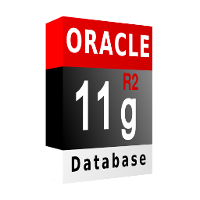
\includegraphics[scale=1]{oracle_11g}}} &
            \multicolumn{1}{c}{\textbf{
\includegraphics[scale=1]{ms_sql}}} &
            \multicolumn{1}{c}{\textbf{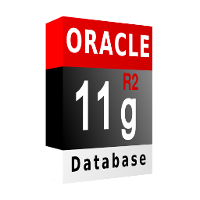
\includegraphics[scale=1]{oracle_11g}}} &
            \multicolumn{1}{c}{\textbf{
\includegraphics[scale=1]{ms_sql}}} &
            \multicolumn{1}{c}{\textbf{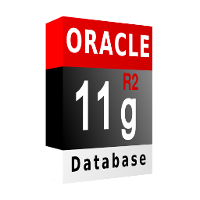
\includegraphics[scale=1]{oracle_11g}}} &
            \multicolumn{1}{c}{\textbf{
\includegraphics[scale=1]{ms_sql}}} \\
            \multicolumn{1}{c}{Einschränkung} &
            \multicolumn{2}{c}{INSERT} &
            \multicolumn{2}{c}{UPDATE} &
            \multicolumn{2}{c}{DELETE} \\
            \hline
        }
        \tabletail{
            \hline
        }
        \tablelasttail {
            \hline
        }
        \begin{supertabular}{|p{9cm}|c|c|c|c|c|c|}
            Es dürfen keine Aggregatfunktionen (COUNT, SUM, MAX, MIN, AVG) in der View genutzt werden. & X & X & X & X & X & X \\
            \hline
            Die View darf keine GROUP BY-Klausel enthalten. & X & X & X & X & X & X \\
            \hline
            Die View darf das DISTINCT-Schlüsselwort nicht benutzen. & X & X & X & X & X & X\\
            \hline
            Die View darf keine berechneten Ausdrücke aufweisen. & X & X & X & X & & \\
            \hline
            Die View darf keine Pseudospalten enthalten & X & & X & & X & \\
            \hline
            Die View darf keinen Join enthalten. & X & X & & & X & X \\
            \hline
            Alle mit NOT NULL markierten Spalten der Basistabelle müssen im INSERT-Statement berücksichtigt werden. & X & X & & & & \\
            \hline
            Der Einfüge- bzw. Änderungsvorgang muss, falls eine CHECK-Option in der View vorhanden ist (siehe \abschnitt{CHECK}), den Vorgaben der WHERE-Klausel der Abfrage genügen. & X & X & X & X & & \\
            \hline
            Die View darf keine READ ONLY-Option (siehe \abschnitt{READONLY}) enthalten. & X & & X & & &\\
        \end{supertabular}
    \end{small}
\end{center}
\subsubsection{Die Einschränkung WITH CHECK OPTION}
\label{CHECK}
Bei der Erstellung einer View kann eine zusätzliche Einschränkung mit angegeben werden, die sogenannte \languageorasql{CHECK OPTION}. Diese schränkt den Nutzer dahingehend ein, dass nur noch solche Datensätze geändert werden können, die auch in der View zu sehen sind.
\begin{lstlisting}[language=oracle_sql,caption={Ein Experiment mit den CHECK OPTION},label=sql08_35]
CREATE VIEW v_Mitarbeiter AS
  SELECT *
  FROM   Mitarbeiter
  WHERE  Bankfiliale_ID = 5;

INSERT INTO v_Mitarbeiter
VALUES (666, 'Florian', 'Weidinger', 12, 8, TO_DATE('01.03.1988', 'DD.MM.YYYY'), 
        '38B546C1-CDF-36A7B97', 1500, 'Abendrot Gase', '13', '39444',
        'Hecklingen', 20);

1 row inserted

ROLLBACK;
          \end{lstlisting}
Obwohl die \WHERE-Klausel der View \identifier{v\_Mitarbeiter} die Anzeige auf die Bankfiliale mit der ID fünf einschränkt, kann trotzdem ein Datensatz in die Bankfiliale Nummer acht eingefügt werden.

Um die DML-Möglichkeiten der View \identifier{v\_Mitarbeiter} einzuschränken, wird im nächsten Beispiel die \languageorasql{CHECK}-Option angewendet.
\begin{lstlisting}[language=oracle_sql,caption={Ein Experiment mit der CHECK OPTION in Oracle},label=sql08_36]
CREATE VIEW v_Mitarbeiter AS
  SELECT *
  FROM   Mitarbeiter
  WHERE  Bankfiliale_ID = 5
WITH CHECK OPTION;

INSERT INTO v_Mitarbeiter
VALUES (666, 'Florian', 'Weidinger', 12, 8, TO_DATE('01.03.1988', 'DD.MM.YYYY'),
        '38B546C1-CDF-36A7B97', 1500, 'Abendrot Gase',
        '13', '39444', 'Hecklingen', 20);

INSERT INTO v_Mitarbeiter
         *
FEHLER in Zeile 1:
ORA-01402: Verletzung der where-Klausel einer View with check option
          \end{lstlisting}
Da jetzt die \languageorasql{CHECK}-Option genutzt wurde, reagiert das DBMS mit einer Fehlermeldung auf DML-Statements, die sich auf \identifier{v\_Mitarbeiter} beziehen und nicht der \WHERE-Klausel der View entsprechen.
\begin{lstlisting}[language=ms_sql,caption={Ein Experiment mit der CHECK OPTION in SQL Server},label=sql08_37]
CREATE VIEW v_Mitarbeiter
AS
  SELECT *
  FROM   Mitarbeiter
  WHERE  Bankfiliale_ID = 5
WITH CHECK OPTION;

INSERT INTO v_Mitarbeiter
VALUES (666, 'Florian', 'Weidinger', 12, 8,
        CONVERT(DATETIME2, '01.03.1988', 104),
        '38B546C1-CDF-36A7B97', 1500, 'Abendrot Gase',
        '13', '39444', 'Hecklingen', 20);

Meldung 550, Ebene 16, Status 1, Zeile 1
Fehler beim Einf&ü&gen oder Aktualisieren, da die Zielsicht WITH CHECK OPTION
angibt oder sich auf eine Sicht erstreckt, die WITH CHECK OPTION angibt,
und mindestens eine Ergebniszeile nicht der CHECK OPTION-Einschr&ä&nkung
entsprach.
          \end{lstlisting}
\subsubsection{Die Einschränkung WITH READ ONLY - Oracle}
\label{READONLY}
Die \languageorasql{READ ONLY}-Option für Views ermöglicht es, einem Nutzer den Schreibzugriff auf eine View zu verbieten. Die View kann somit nur noch lesend genutzt werden.
\begin{lstlisting}[language=oracle_sql,caption={Eine View mit mit READ ONLY Option erstellen},label=sql08_38]
CREATE VIEW v_Mitarbeiter
AS
  SELECT *
  FROM   Mitarbeiter
WITH READ ONLY;
          \end{lstlisting}
Versucht ein Nutzer trotzdem mit einem DML-Statement auf die View zuzugreifen, wird er mit einer Fehlermeldung abgewiesen.
\clearpage
\begin{lstlisting}[language=oracle_sql,caption={Daten in eine READ ONLY View einfügen schlägt fehl},label=sql08_39]
INSERT INTO v_Mitarbeiter
VALUES (666, 'Florian', 'Weidinger', 12, 8,
        TO_DATE('01.03.1988', 'DD.MM.YYYY'),
        '38B546C1-CDF-36A7B97', 1500, 'Abendrot Gase',
        '13', '39444', 'Hecklingen', 20);

INSERT INTO v_Mitarbeiter
*
FEHLER in Zeile 1:
ORA-42399: cannot perform a DML operation on a read-only view
          \end{lstlisting}
Um diese Option wieder von der View zu nehmen, muss die View neu erstellt werden (siehe \abschnitt{alterview})
\subsection{Views ändern}
\label{alterview}
Müssen an einer View Veränderungen vorgenommen werden, bedeutet dies immer, dass die View neu erstellt werden muss. Oracle und SQL Server kennen hierzu unterschiedliche Wege:
\begin{itemize}
    \item In Oracle wird die \languageorasql{CREATE VIEW}-Klausel erweitert: \languageorasql{CREATE OR REPLACE VIEW}.
    \item SQL Server benutzt hierfür die \languagemssql{ALTER VIEW}-Anweisung.
\end{itemize}
Die beiden Beispiele \beispiel{sql08_40} und \beispiel{sql08_41} zeigen, wie in Oracle und SQL Server eine Viewdefinition geändert werden kann.
\begin{lstlisting}[language=oracle_sql,caption={Eine View ändern in Oracle},label=sql08_40]
-- Zuerst wird die View erstellt
CREATE VIEW v_Mitarbeiter
AS
  SELECT *
  FROM   Mitarbeiter
WITH READ ONLY;

-- Dann wird sie geaendert
CREATE OR REPLACE VIEW v_Mitarbeiter
AS
  SELECT *
  FROM   Mitarbeiter;
        \end{lstlisting}
\clearpage
Und nun SQL Server.
\begin{lstlisting}[language=ms_sql,caption={Eine View ändern in SQL
Server},label=sql08_41]
-- Zuerst wird die View erstellt
CREATE VIEW v_Mitarbeiter
AS
  SELECT *
  FROM   Mitarbeiter;

-- Dann wird sie ge&ä&ndert
ALTER VIEW v_Mitarbeiter
AS
  SELECT *
  FROM   Mitarbeiter
  WHERE  Bankfiliale_ID = 5;
        \end{lstlisting}
\subsection{Views löschen}
Zum Löschen von Views gibt es das Kommando \languageorasql{DROP VIEW}.
\begin{lstlisting}[language=ms_sql,caption={Eine View löschen},label=sql08_42]
DROP VIEW viw_countries;
        \end{lstlisting}
